\section{Алгоритм работы распределителя памяти zsmalloc}

zsmalloc -- специально спроектированный распределитель памяти (далее -- аллокатор) для работы в ситуациях, когда в системе критически мало памяти \cite{zsmalloc}. Данный аллокатор так же работает с физически непрерывными участками памяти, но максимальный участок памяти, который он может выделить, ограничен размером \texttt{PAGE\_SIZE}. Данный аллокатор базируется поверх алгоритма buddy-системы \cite{kernel-development}. 

\subsection{Функции для работы с распределителем}

Аллокатор предоставляет специальное API  \cite{bootlin}, описанное в листинге \ref{code:zsmalloc_api}.

\begin{code}
	\captionof{listing}{API для работы с zsmalloc}
	\label{code:zsmalloc_api}
	\inputminted
	[
	frame=single,
	framerule=0.5pt,
	framesep=20pt,
	fontsize=\small,
	tabsize=4,
	linenos,
	numbersep=5pt,
	xleftmargin=10pt,
	]
	{c}
	{code/zsmalloc_api.c}
\end{code}

Рассмотрим подробнее данные функции:

\begin{itemize}
	\item \texttt{zs\_create\_pool} -- создать пулл, в котором в дальнейшем будут выделяться объекты;
	\item \texttt{zs\_destroy\_pool} -- уничтожить пулл объектов;
	\item \texttt{zs\_malloc} -- выделить объект размером \texttt{size} внутри пулла \texttt{pool}. Возвращает целое без знаковое число, обычно именуемое \texttt{handle};
	\item \texttt{zs\_free} -- освободить ранее выделенный функцией \texttt{zs\_malloc} объект;
	\item \texttt{zs\_map\_object} -- получить соответствие между числом (\texttt{handle}), которое вернула функция \texttt{zs\_malloc} и указателем на выделенную областью памяти, то есть получить указатель на начало выделенного аллокатором участка памяти. Из-за внутренних особенностей архитектуры zsmalloc, в один момент времени может быть получено не более одного соответствия между \texttt{handle} и указателем на выделенную область памяти;
	\item \texttt{zs\_unmap\_object} -- убрать соответствие между \texttt{handle} и адресом на выделенную акллокатором память. После вызова этой функции, обращаться к ранее выделенному участку памяти запрещено. 
\end{itemize}

\subsection{Дескриптор zspage}

Единицей диспетчеризации аллокатора является структура данных, называемая zspage, которая описывается соответствующей структурой \texttt{struct zspage}, поля которой представлены в листинге \ref{code:zspage}. 

\pagebreak

\begin{code}
	\captionof{listing}{Структура \texttt{struct zspage}}
	\label{code:zspage}
	\inputminted
	[
	frame=single,
	framerule=0.5pt,
	framesep=20pt,
	fontsize=\small,
	tabsize=4,
	linenos,
	numbersep=5pt,
	xleftmargin=10pt,
	]
	{c}
	{code/zspage.c}
\end{code}

zspage -- это связанный список из объеденных страниц \texttt{struct page}, которые указывают друг на друга с помощью поля \texttt{index}. zspage -- это структура данных, которая предоставляет хранилище для объектов одинакового размера, размещенных в памяти друг за другом, основываясь на структуре \texttt{struct page}. Таким образом, объект может находиться сразу на двух страница одновременно: часть байт на странице с индексом $i$, а оставшаяся часть на странице $i + 1$. Суть заключается в том, чтобы подобрать такое количество страниц памяти \texttt{struct page}, чтобы максимально вместительно разместить в памяти объекты размером $n$.

Рассмотрим подробнее, поля структуры описанные в листинге \ref{code:zspage}:

\begin{itemize}
	\item c помощью анонимный структуры (битовое поле), описываются различные флаги необходимые для работы;
	\item \texttt{inuse} -- количество занятых объектов на странице \texttt{zspage};
	\item \texttt{freeobj} -- количество свободных объектов;
	\item \texttt{first\_page} -- указатель на первую странице в связанном списке страниц;
	\item \texttt{list} -- список структур \texttt{zspage};
	\item \texttt{pool} -- указатель на пул страниц, описание которого приводится далее.
\end{itemize}

На рисунке \ref{fig:zspage} представлена схема взаимодействия структуры\\ \texttt{struct zspage} и структур \texttt{struct page}.

\begin{figure}[h]
	\centering
	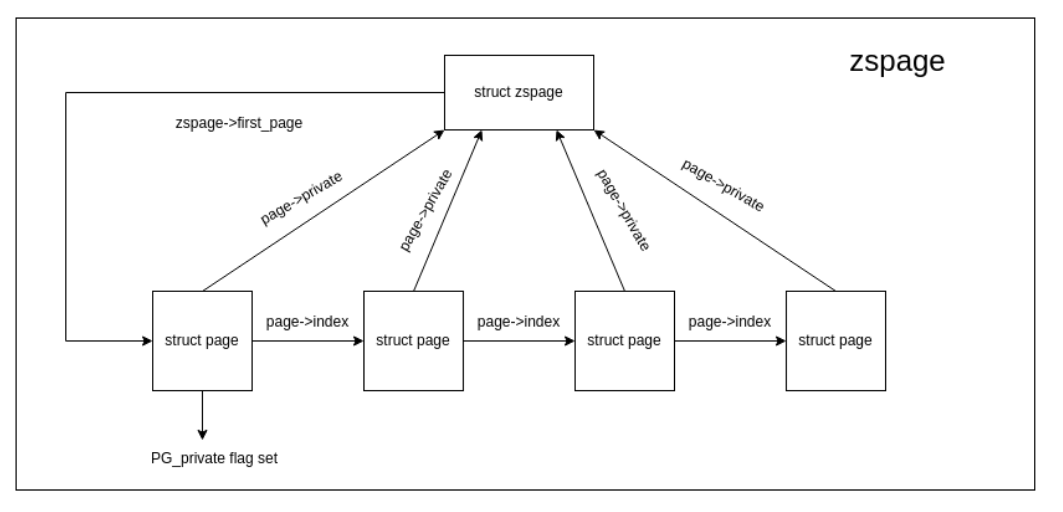
\includegraphics[width=0.95\textwidth]{img/zspage.png}
	\caption{Схематическое описание структуры данных zspage}
	\label{fig:zspage}
\end{figure}

Структуры \texttt{struct page} связаны друг с другом при помощи поля \texttt{index}, которое является указателем на начало каждой последующей страницы списка. Для вычисления, к какой именно структуре zspage страница относится, используется поле \texttt{private}, являющееся указателем на соответствующую структуру \texttt{struct zspage}. У первой странице в списке установлен флаг \texttt{PG\_private}, а так же структура \texttt{struct zspage} имеет указатель на эту страницу. Максимум в списке может быть 4 страницы, минимум -- одна.

\subsection{Дескриптор объектов}

На рисунке \ref{fig:zspage_mem} представлено расположение выделяемых объектов в памяти.

\begin{figure}[h]
	\centering
	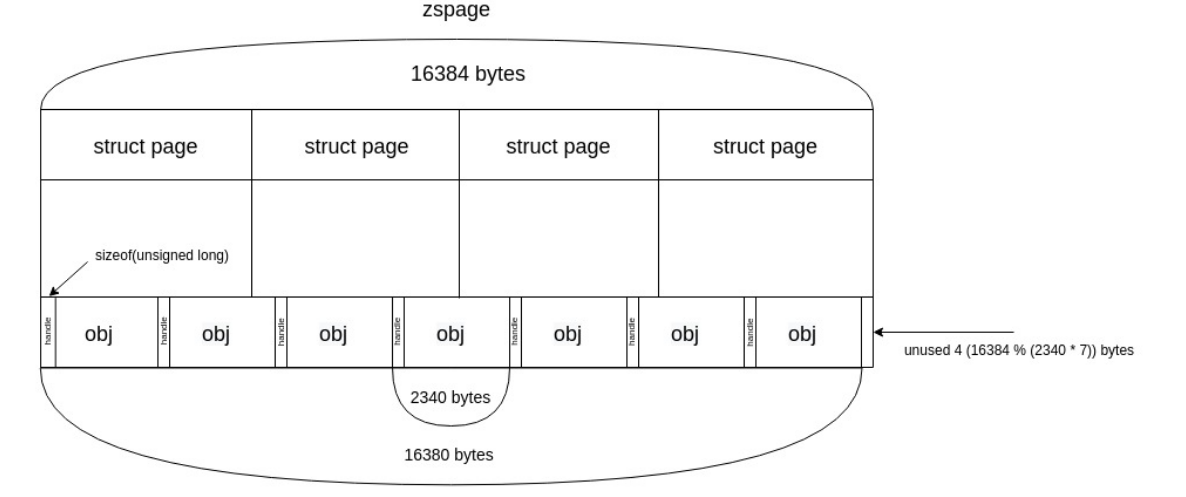
\includegraphics[width=\textwidth]{img/zspage_mem.png}
	\caption{Расположение объектов, хранящихся в zspage, в памяти}
	\label{fig:zspage_mem}
\end{figure}

Объекты (обозначены именем \texttt{obj}), находятся в памяти друг за другом. Перед каждым находится его дескриптор, размер которого соответствует\\ \texttt{sizeof(unsigned long)}. Это некоторое целое, безналичное число, которое кодирует положение данного объекта в памяти. В случае, если объект не выделен, дескриптор указывает на следующий свободный объект, тем самым формируя список свободных объектов внутри zspage. 

На рисунке \ref{fig:handle} представлено описание дескриптора, описывающего запрашиваемые у аллокатора объекты. 

\begin{figure}[h]
	\centering
	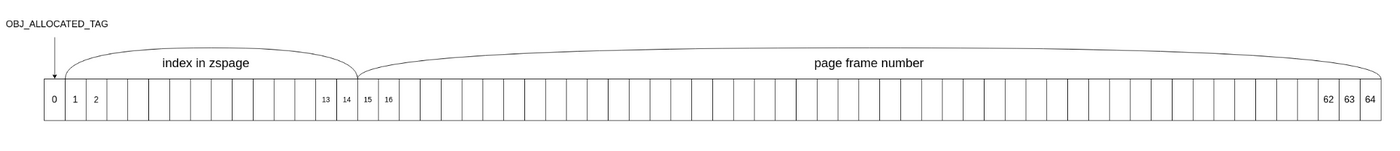
\includegraphics[width=\textwidth]{img/handle.png}
	\caption{Дескриптор объекта}
	\label{fig:handle}
\end{figure}

Дескриптор представляется из себя целое число, состоящее из \\ \texttt{sizeof(unsigned long)} байт. Для простоты изложения, его размер указан в качестве 8 байт (64 бита). 

Первый бит является тегом, позволяющим определить, свободен ли объект. Если первый бит установлен в 0, это значит, что область памяти, находящаяся за дескриптором, не используется. В таком случае, оставшиеся 63 бита являются указателем на следующий свободный участок памяти. В обратном случае (то есть объект уже кем-то используется) биты с 1 по 14 описывают индекс объекта внутри zspage. Оставшиеся биты являются порядковым номером страницы \texttt{struct page} в глобальном массиве \texttt{mem\_map}, который был описан ранее. При выделении объекта, функция \texttt{zs\_malloc} возвращает данный дескриптор.

\subsection{Хранение страниц zspage}

Страницы zspage связаны друг с другом с помощью связанного списка. Для каждого размера объекта, в системе существует 4 связанных списка, хранящие страницы zspage:

\begin{itemize}
	\item \texttt{ZS\_EMPTY} -- список, хранящий страницы zspage в которых все объекты свободны;
	\item \texttt{ZS\_FULL} -- список zspage, в которых все объекты заняты;
	\item \texttt{ZS\_ALMOST\_EMPTY} -- список zspage, в которых количество занятых объектов не превышает $\frac{3 * obj}{4}$, где \texttt{obj} -- общее количество объектов в странице;
	\item \texttt{ZS\_ALMOST\_FULL} -- список zspage, не попавшими ни в один из вышеперечисленных списков.
\end{itemize}

На рисунке \ref{fig:fullness_group} представлено взаимодействие списков \texttt{ZS\_EMPTY}, \texttt{ZS\_FULL}, \texttt{ZS\_ALMOST\_EMPTY}, \texttt{ZS\_ALMOST\_FULL} и страниц zspage. 

\begin{figure}[h]
	\centering
	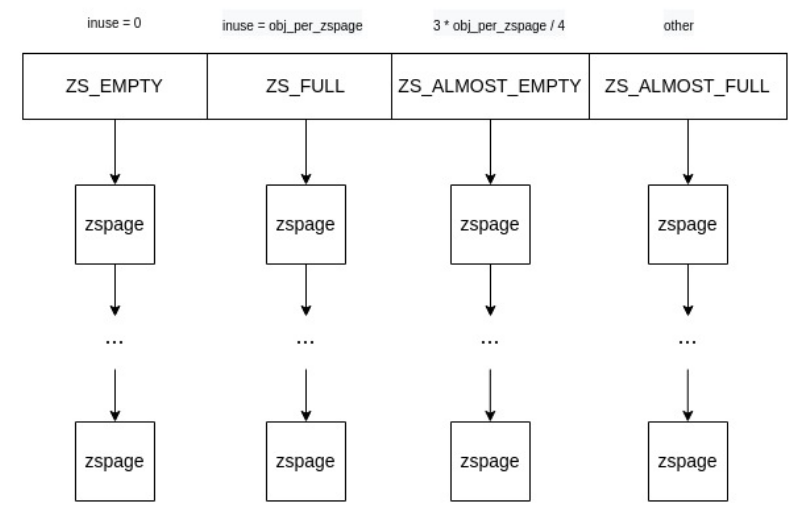
\includegraphics[width=\textwidth]{img/fullness_group.png}
	\caption{Взаимодействие zspage}
	\label{fig:fullness_group}
\end{figure}

Для эффективного размещения объектов разного размера в памяти, используется структуры данных называемые size class и zspool, в исходном коде описываемые соответственно структурами \texttt{struct size\_class} и {struct zs\_pool} (см. листинги \ref{code:size_class} -- \ref{code:zs_pool}).

\pagebreak

\begin{code}
	\captionof{listing}{Структура \texttt{struct size\_class}}
	\label{code:size_class}
	\inputminted
	[
	frame=single,
	framerule=0.5pt,
	framesep=20pt,
	fontsize=\small,
	tabsize=4,
	linenos,
	numbersep=5pt,
	xleftmargin=10pt,
	]
	{c}
	{code/size_class.c}
\end{code}

Структура данных size\_class предназначена для хранения всех объектов размером \texttt{size}. Данная структура данных хранит в себе указатели на  четыре списка, описанных ранее, которые в свою очередь указывают на страницы zspage. Поле \texttt{objs\_per\_zspage} хранит в себе количество объектов, размещаемых в страницах zspage для данного size class, а в поле \texttt{page\_per\_zspage} хранится количество страниц памяти, используемых внутри zspage.

\begin{code}
	\captionof{listing}{Структура \texttt{struct zs\_pool}}
	\label{code:zs_pool}
	\inputminted
	[
	frame=single,
	framerule=0.5pt,
	framesep=20pt,
	fontsize=\small,
	tabsize=4,
	linenos,
	numbersep=5pt,
	xleftmargin=10pt,
	]
	{c}
	{code/zs_pool.c}
\end{code}

zspool -- самая <<верхняя>> структура данных, используемая в алгоритме работы аллокатора zsmalloc. Данная структура хранит в себе массив типа \\ \texttt{size\_class}, таким образом, каждому пулу принадлежит \texttt{ZS\_SIZE\_CLASSES} соответствующих структур. Суть заключается в том, что каждый size\_class отличается от предыдущего размером объектов, которые он хранит. Таким образом, самый size\_class хранит объекты размером \texttt{PAGE\_SIZE}, второй объекты размером \texttt{PAGE\_SIZE - C}, третий \texttt{PAGE\_SIZE - 2 * C} и так далее. На данный момент, $C = 8$, что позволяет создать до 255 size class, при размере страницы 4 Кб. При запросе у аллокатора участка памяти размером $n$ байт, $n$ будет округлено до ближайшего размера size class. Несмотря на то, что размер будет округлен, благодаря большому количеству size class, количество на самом деле неиспользуемых байт будет минимально возможным.  Такой подход позволяет максимально эффективно распределять и управлять участками памяти.

На рисунке \ref{fig:zsmalloc_full} представлено взаимодействие всех описанных в этом разделе структур данных.

\begin{figure}[h]
	\centering
	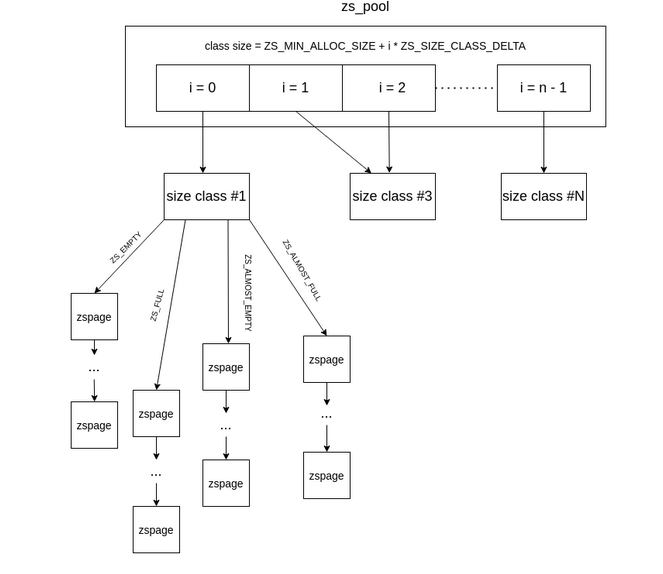
\includegraphics[width=\textwidth]{img/zsmalloc_full.png}
	\caption{Взаимодействие структур данных аллокатора zsmalloc}
	\label{fig:zsmalloc_full}
\end{figure}

\section{Метод объединения одинаковых объектов}

В данном разделе будет разработан метода объединения одинаковых объектов: изложены особенности метода, представлена схема используемых алгоритмов и описаны структуры данных используемые в разработанном методе.

\subsection{Особенности метода}

Суть метода заключается в сканировании всех объектов, хранящихся в дескрипторе $zs\_pool$, вычисления и сохранения хэш-значения в хэш-таблицу \cite{hash-table}. В случае, если вычисленное хэш-значение, например для объекта $i$, совпадает с хэш-значением одного из объектов который был обработан ранее, например объекта $j$, необходимо сделать так, чтобы у объекта $i$ теперь был такой же дескриптор что и объекта $j$. Участок памяти, на который дескриптор объекта $i$ нужно освободить.

Ниже представлены особенности метода объединения одинаковых объектов, которые необходимо предусмотреть при разработке метода:

\begin{itemize}
	\item дескриптор типа $size\_class$ хранит объекты одинакового размера. Например, в $size\_class_{k}$ расположены объекты размером $k$, а в $size\_class_{t}$ хранятся объекты размером $t$. Таким образом, нужно обходить и строить хэш-таблицу не для всех объектов $zs\_pool$, а для каждого $size\_class$ отдельно;
	
	\item для того чтобы не освободить область памяти, на которую ссылается дескриптор другого объект, необходимо хранить счётчик ссылок. Для этого можно использовать красно-черное дерево \cite{rbtree}: ключом будет являться дескриптор объекта, а значением -- количество ссылок на этот объект;
	
	\item стоит учесть, что код ядра Linux может исполняться в нескольких потоках и для того чтобы не повредить структуры данных, необходимо использовать средства синхронизации потоков. Код аллокатора zsmalloc может исполняться в атомарном контексте, что означает что можно использовать только spin-блокировки \cite{spinlock};
	
	\item элементы дерева и хэш-таблицы будут выделяться очень часто, причем их размер всегда будет одинаковым. Таким образом, для выделения этих объектов можно использовать Slab-кэши \cite{slab-cache}. 
\end{itemize}

\subsection{Структуры данных}

Для хранения хэш-значений объектов необходимо использовать хэш-таблицу. В данной реализации будет использована хэш-таблица с использованием цепочек. В ядре Linux для реализации таких таблиц существует специальная структура типа \texttt{struct hlist\_node}.

В листинге \ref{code:hash-table} представлена структура \texttt{struct hash\_table}, которая является дескриптором хэш-таблицы.

\begin{code}
	\captionof{listing}{Структура \texttt{struct hash\_table}}
	\label{code:hash-table}
	\inputminted
	[
	frame=single,
	framerule=0.5pt,
	framesep=20pt,
	fontsize=\small,
	tabsize=4,
	linenos,
	numbersep=5pt,
	xleftmargin=10pt,
	]
	{c}
	{code/hash_table.c}
\end{code}

\begin{itemize}
	\item \texttt{table} -- массив списков, хранящий элементы таблицы;
	\item \texttt{cachep} -- указатель на Slab-кэш, с помощью которого выделяются объекты для таблицы;
	\item \texttt{size} -- количество элементов, хранящихся в таблице;
\end{itemize}

\pagebreak

В листинге \ref{code:hash-node} описана структура \texttt{struct obj\_hash\_node}, которая является ячейкой хэш-таблицы.

\begin{code}
	\captionof{listing}{Структура \texttt{struct obj\_hash\_node}}
	\label{code:hash-node}
	\inputminted
	[
	frame=single,
	framerule=0.5pt,
	framesep=20pt,
	fontsize=\small,
	tabsize=4,
	linenos,
	numbersep=5pt,
	xleftmargin=10pt,
	]
	{c}
	{code/hash_node.c}
\end{code}

\begin{itemize}
	\item \texttt{handle} -- дескриптор объекта;
	\item \texttt{next} -- следующий элемент в списке (необходимо для решения коллизий).
\end{itemize}

Для хранения ссылок на объект будет использоваться красно-черное дерево, которое так же уже реализовано в ядре Linux. Необходимо лишь описать дескриптор узла дерева (листинг \ref{code:rbtree-node}).

\begin{code}
	\captionof{listing}{Структура \texttt{struct fold\_rbtree\_node}}
	\label{code:rbtree-node}
	\inputminted
	[
	frame=single,
	framerule=0.5pt,
	framesep=20pt,
	fontsize=\small,
	tabsize=4,
	linenos,
	numbersep=5pt,
	xleftmargin=10pt,
	]
	{c}
	{code/rbtree_node.c}
\end{code}

\begin{itemize}
	\item \texttt{node} -- родительская структура ячейки дерева, в которую встраиваются наши данные.
	\item \texttt{key} -- ключ, по которому можно идентифицировать узел - совпадает с дескриптором объекта;
	\item \texttt{cnt} -- количество ссылок на объект.
\end{itemize}

\subsection{Формальное описание метода}

На рисунке \ref{fig:idef0-0} представлена IDEF0-диаграмма разрабатываемого метода.

\begin{figure}[h]
	\centering
	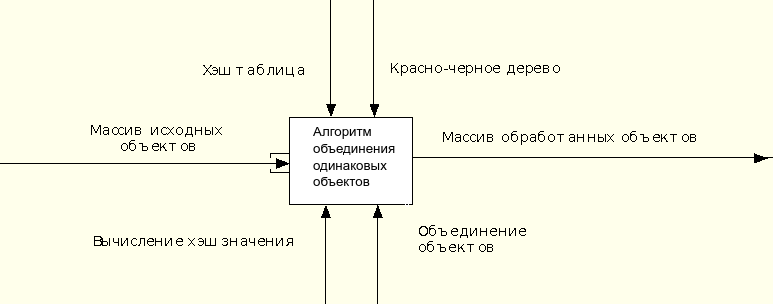
\includegraphics[width=\textwidth]{img/idef0-0.png}
	\caption{IDEF0-диаграмма разрабатываемого метода}
	\label{fig:idef0-0}
\end{figure}

На рисунке \ref{fig:idef0-1} представлена детализированная IDEF0-диаграмма разрабатываемого метода.

\begin{figure}[h]
	\centering
	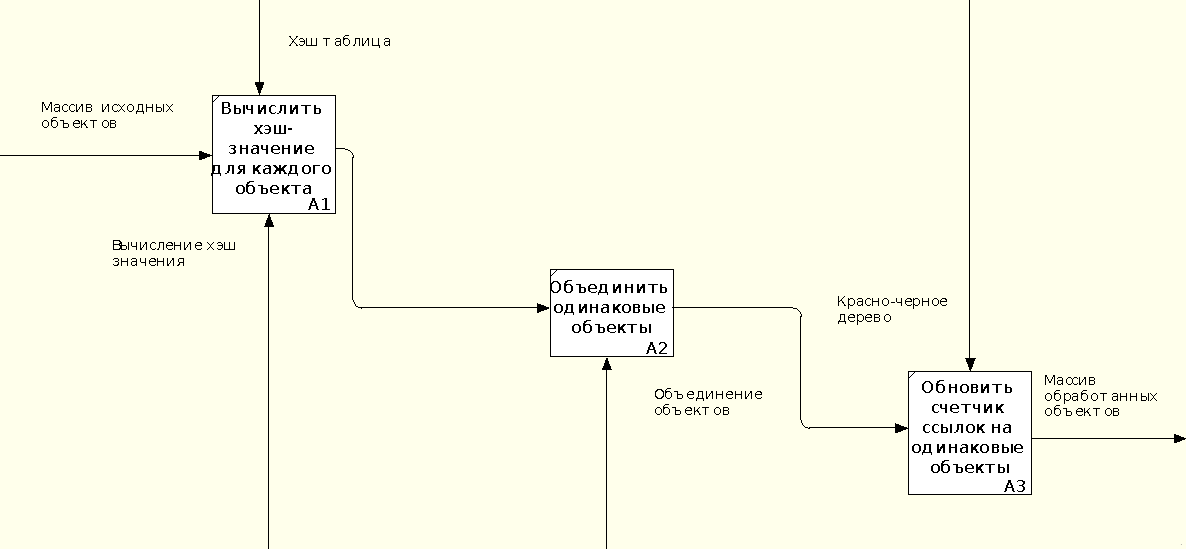
\includegraphics[width=\textwidth]{img/idef0-1.png}
	\caption{Детализированная IDEF0-диаграмма разрабатываемого метода}
	\label{fig:idef0-1}
\end{figure}

\subsection{Описание используемых алгоритмов}

\subsubsection{Алгоритм вычисления хэш значений для объектов}

На рисунке \ref{fig:scheme-0} представлена схема алгоритма вычисления хэш значений для каждого объекта, которые хранятся внутри распределителя памяти zsmalloc.

\begin{figure}[h]
	\centering
	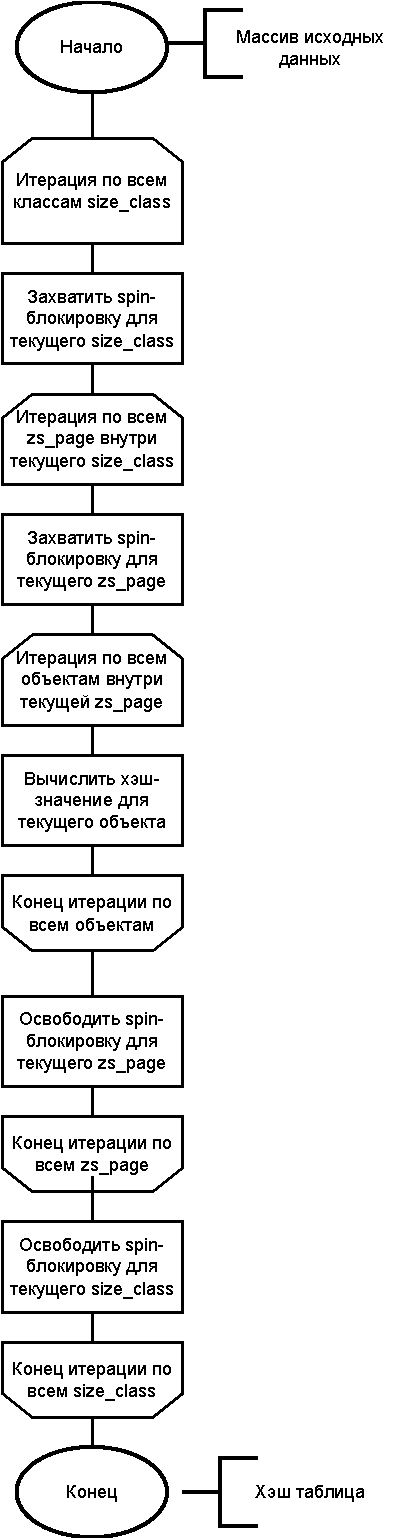
\includegraphics[scale=0.6]{img/scheme-0.pdf}
	\caption{Схема алгоритма вычисления хэш значений для объектов}
	\label{fig:scheme-0}
\end{figure}

\subsubsection{Алгоритм объединения одинаковых объектов}

На рисунке \ref{fig:scheme-1} представлена схема алгоритма объединения одинаковых объектов.

\begin{figure}[h]
	\centering
	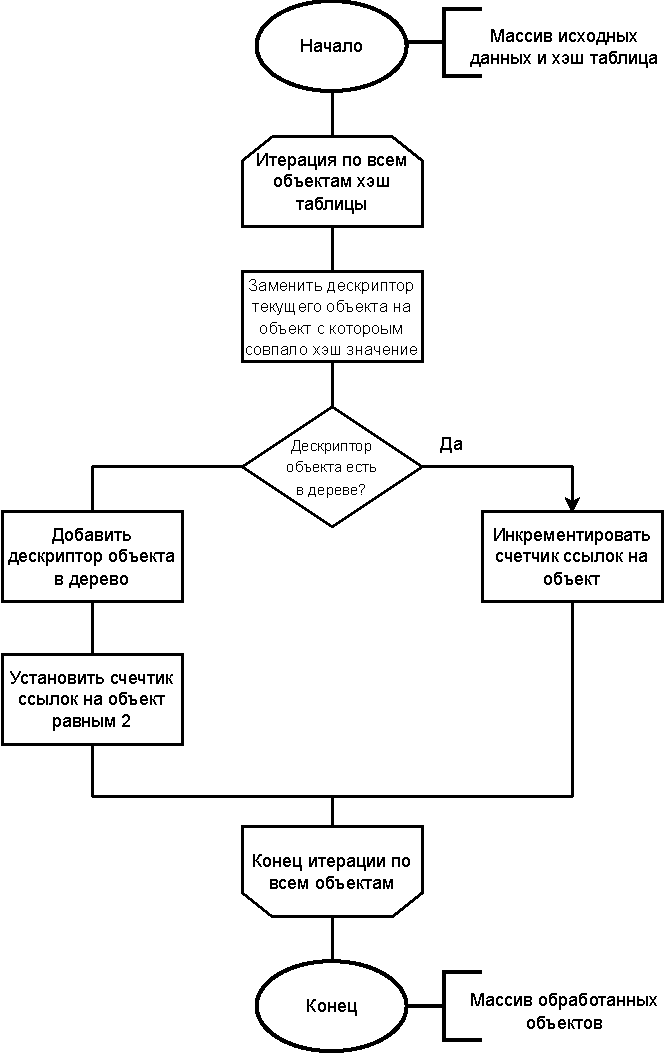
\includegraphics[scale=1]{img/scheme-1.pdf}
	\caption{Схема алгоритма объединения одинаковых объектов}
	\label{fig:scheme-1}
\end{figure}

\pagebreak
